%! TEX root = main.tex
The overall run times for the steady, unsteady, and data-driven cases are about 28 hours, 31 hours, and 33.5 hours.
The PetIBM simulation, on the other hand, took around 1.7 hours with a 5-generation behind GPU.

Figure \ref{fig:cylinder-re200-train-hist} shows the convergence history of all cases.
\begin{figure}[hbt!]
    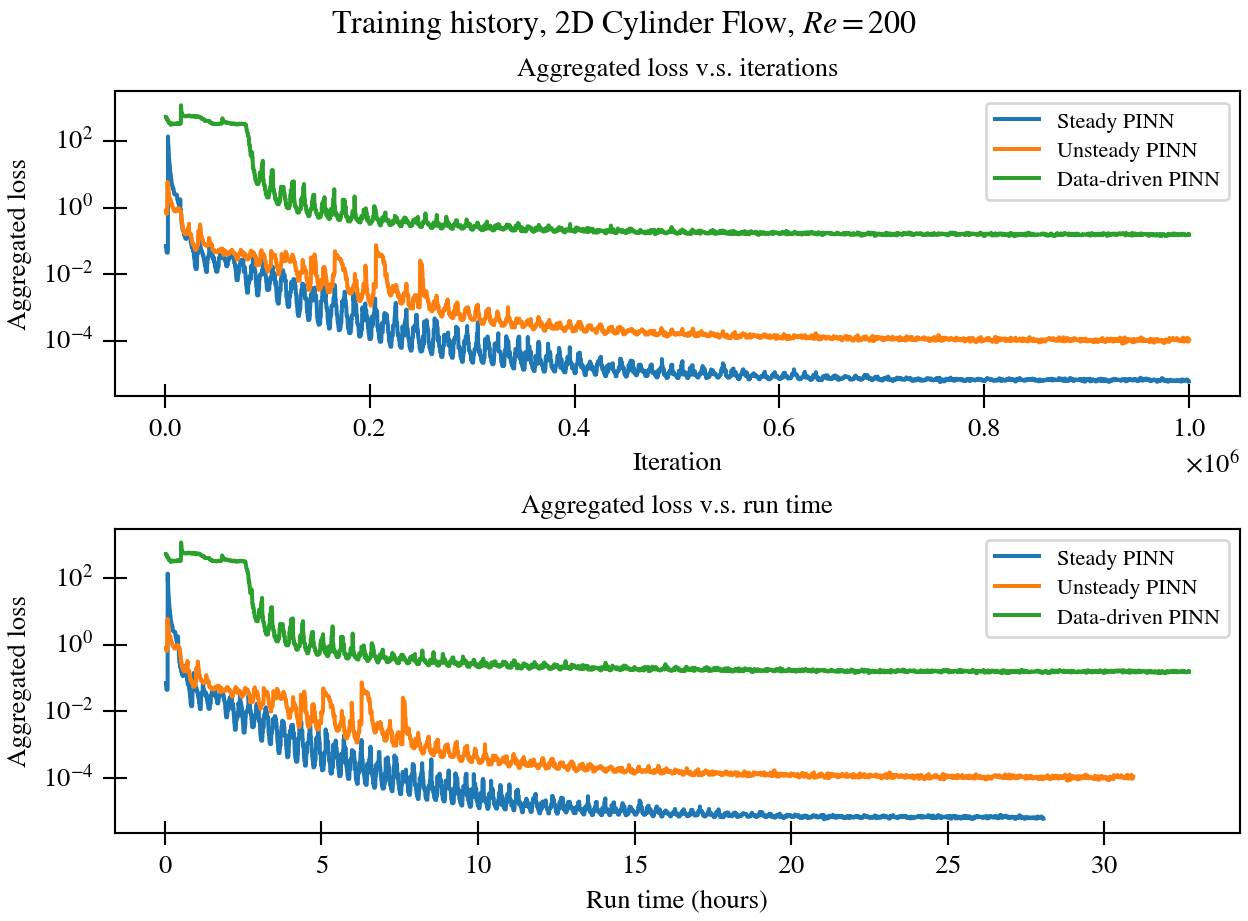
\includegraphics[width=0.9\linewidth]{cylinder-2d-re200/loss-hist}
    \caption{PINNs, 2D Cylinder, $Re=200$: training history}
    \label{fig:cylinder-re200-train-hist}
\end{figure}
One sub-plot is for losses versus iterations, while the other one is against the run times.
The plateaus we observed in the $Re=40$ cases also exist in the unsteady and data-driven cases here.
The steady case does not show any sign of the plateau.
The data-driven does not converge to a loss level as small as that of the other two cases.
However, the aggregated loss of the data-driven case has extra data loss terms, so it is unclear at this point if all loss terms have higher values or only the data loss terms are higher. 

Figure \ref{fig:cylinder-re200-drag-lift} shows the drag and lift coefficients versus simulation time.
\begin{figure}[hbt!]
    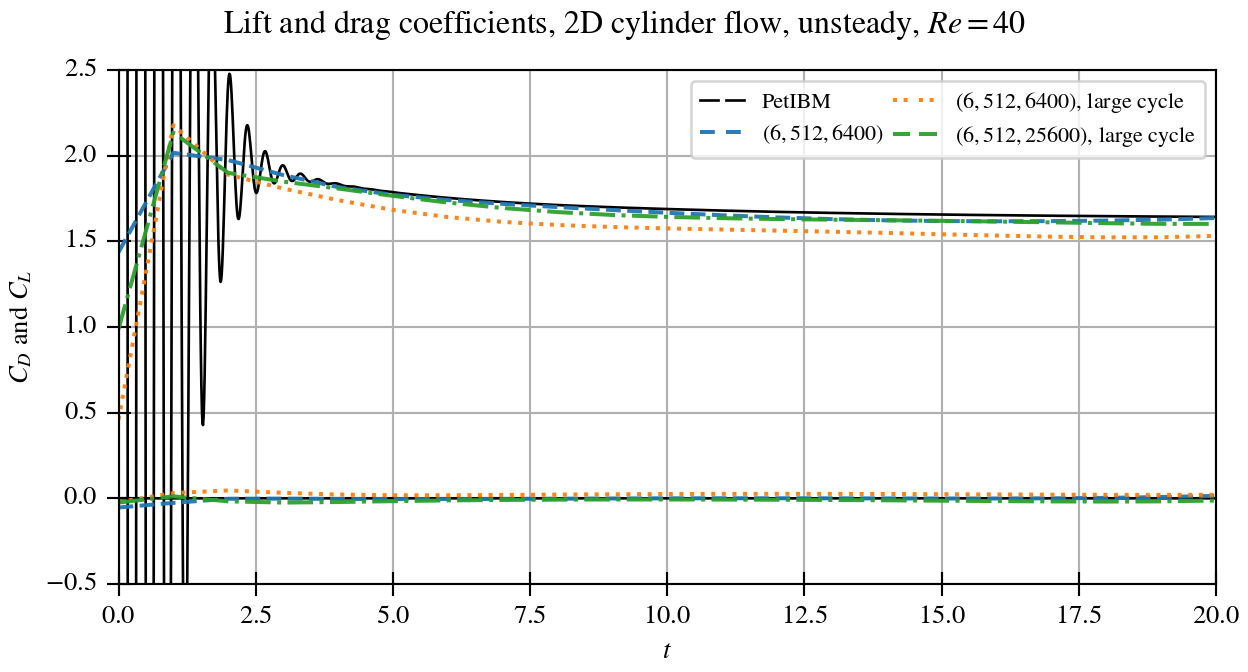
\includegraphics[width=0.9\linewidth]{cylinder-2d-re200/drag-lift-coeffs}
    \caption{PINNs, 2D Cylinder, $Re=200$: drag and lift coefficients}
    \label{fig:cylinder-re200-drag-lift}
\end{figure}
The coefficients from the steady case is just a horizontal line because there is no time variable in this case.
The unsteady case, to our surprise, does not exhibit oscillation, meaning probably no vortex shedding.
Although, it fits well with the PetIBM result before shedding happens (before around $t=75$), including the wake development stage before $t=25$.
Comparing the coefficients between the steady, unsteady, and PetIBM's values before shedding, we believe the unsteady PINN in this particular case behaves just like a steady solver.
This speculation is further supported by the values in table \ref{table:cylinder-2d-re200-cd}, where we compare $C_D$ to both unsteady and steady numerical simulations from literature.
\begin{table}[hbt!]
    \singlespacing
    \begin{threeparttable}[b]
        \begin{tabular}{lcc}
            \toprule
            & $C_D$ \\
            \midrule
            PetIBM & 1.38   \\
            Steady PINN & 0.95 \\
            Unsteady PINN & 0.95 \\
            Deng et al., 2007\cite{deng_hydrodynamic_2007}\tnote{1} & 1.25 \\
            Rajani et al., 2009\cite{Rajani2009}\tnote{1} & 1.34 \\
            Gushchin \& Shchennikov, 1974\cite{gushchin_numerical_1974}\tnote{2} & 0.97 \\
            Fornberg, 1980\cite{fornberg_numerical_1980}\tnote{2} & 0.83 \\
            \bottomrule
        \end{tabular}%
        \begin{tablenotes}
            \footnotesize
            \item [1] Unsteady simulations.
            \item [2] Steady simulations.
        \end{tablenotes}
        \caption[
            PINNs, 2D Cylinder, $Re=200$: validation of drag coefficients%
        ]{%
            PINNs, 2D Cylinder, $Re=200$: validation of drag coefficients.%
            The data-driven case is excluded because it does not have an obvious periodic state nor a steady-state solution.%
        }%
        \label{table:cylinder-2d-re200-cd}
    \end{threeparttable}
\end{table}%

The $C_D$ obtained from the unsteady PINN is the same as the steady PINN and close to those steady CFD simulation results.

As for the data-driven case, its temporal domain is $t\in[125, 200]$, so the coefficients' trajectories start from $t=125$.
The result, again unexpected to us, only exhibits shedding in the time range where we provide data with shedding to the PINN ($t\in[125, 140]$).
This result also shows that data-driven PINNs may be more difficult to train, compared to data-free PINNs and regular data-only model fitting.
Even in the range of provided data, the data-driven case is not able to reach the given maximal $C_L$, and the $C_D$ is obviously off from the given data.
After $t=140$, the trajectories quickly fall back to the no-shedding pattern, though it still deviates from the trajectories of the steady and unsteady PINNs.
Combining the loss magnitude shown in figure \ref{fig:cylinder-re200-train-hist}, the deviation of values may be caused by not enough training.
As figure \ref{fig:cylinder-re200-train-hist} shows data-driven PINN is converged, other optimization techniques or hyperparameter tuning may be required to further reduce the loss.

Nevertheless, we believe not being trained enough only explains why the data-driven case deviates from the given data and the trajectories of the other two cases.
Even with a better optimization and eventually a lower loss, based on the trajectories, we do not believe the shedding will continue after $t=140$.

To examine how the transient flow develops, below we show several snapshots of the flow fields from PetIBM and PINNs:
\begin{enumerate}
    \item Figure \ref{fig:cylinder-re200-contour-steady} shows the flow field obtained from the steady PINN as a reference.
    \item Figures \ref{fig:cylinder-re200-contour-uv-t10} and \ref{fig:cylinder-re200-contour-pwz-t10}: flow at $t=10$. We can see the wake is still developing, and the unsteady PINN visually match the PetIBM. It means the unsteady PINN is indeed an unsteady solver. This time is out of the data-driven PINN's temporal domain.
    \item Figures \ref{fig:cylinder-re200-contour-uv-t50} and \ref{fig:cylinder-re200-contour-pwz-t50}: flow at $t=50$. These figures further confirm that the unsteady PINN matches the PetIBM simulation before shedding.
    \item Figures \ref{fig:cylinder-re200-contour-uv-t140} and \ref{fig:cylinder-re200-contour-pwz-t140}: flow at $t=140$. At this point, the shedding already happened. And $t=140$ is the last snapshot we fed to the data-driven PINN for training. The flow from data-driven PINN shows that it at least is able to qualitatively capture the shedding, which is expected.
    \item Figures \ref{fig:cylinder-re200-contour-uv-t144} and \ref{fig:cylinder-re200-contour-pwz-t144}: flow at $t=144$. Just $4$ unit time from the last snapshot we fed to the data-driven PINN, the data-driven PINN has already stop generating new vortex. The existing vortex can be seen moving toward the boundary, and the wake is gradually recovering to the steady state wake.
    \item Figures \ref{fig:cylinder-re200-contour-uv-t190} and \ref{fig:cylinder-re200-contour-pwz-t190}: flow at $t=190$. Flow field at this time further confirm that the data-driven PINN's behavior is leaning toward that of the unsteady PINN, which is itself behaving like a steady state solver.
\end{enumerate}

\begin{figure}[hbt!]
    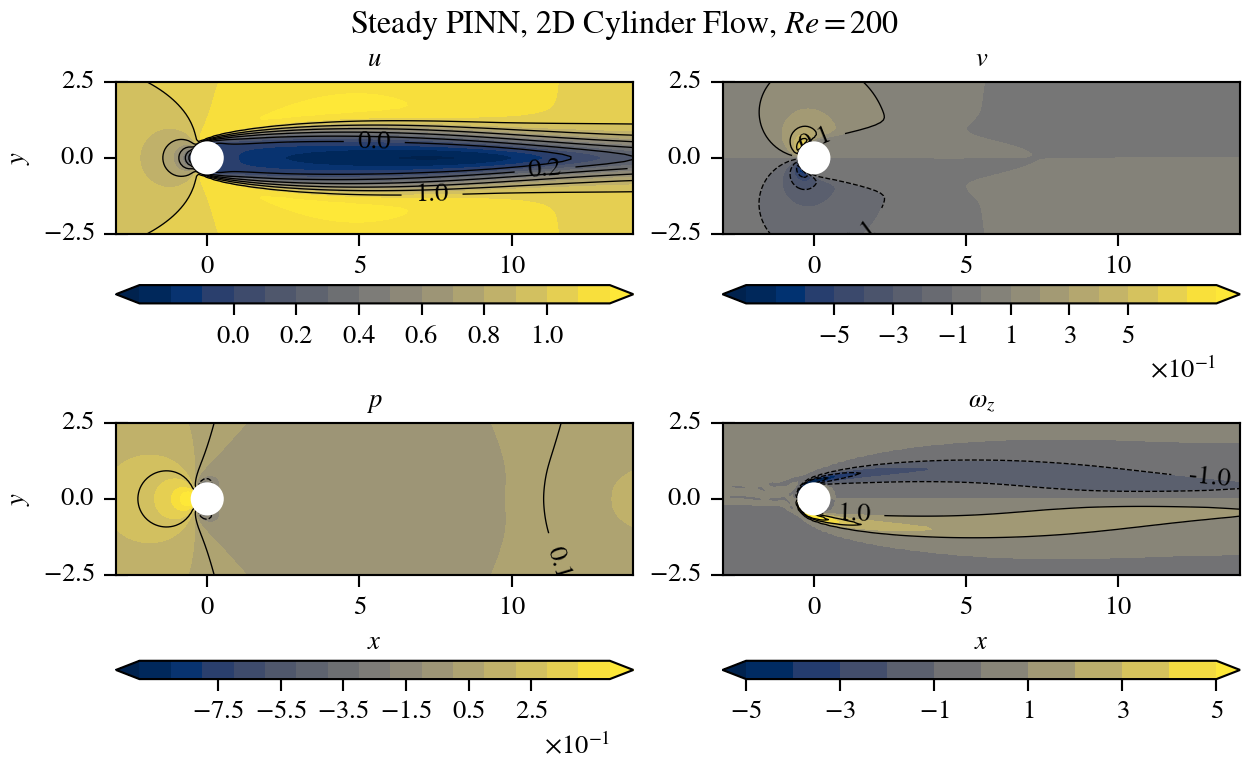
\includegraphics[width=0.9\linewidth]{cylinder-2d-re200/contour-comparison-steady}
    \caption{PINNs, 2D Cylinder, $Re=200$: flow field contours for steady PINN}
    \label{fig:cylinder-re200-contour-steady}
\end{figure}

\begin{figure}[hbt!]
    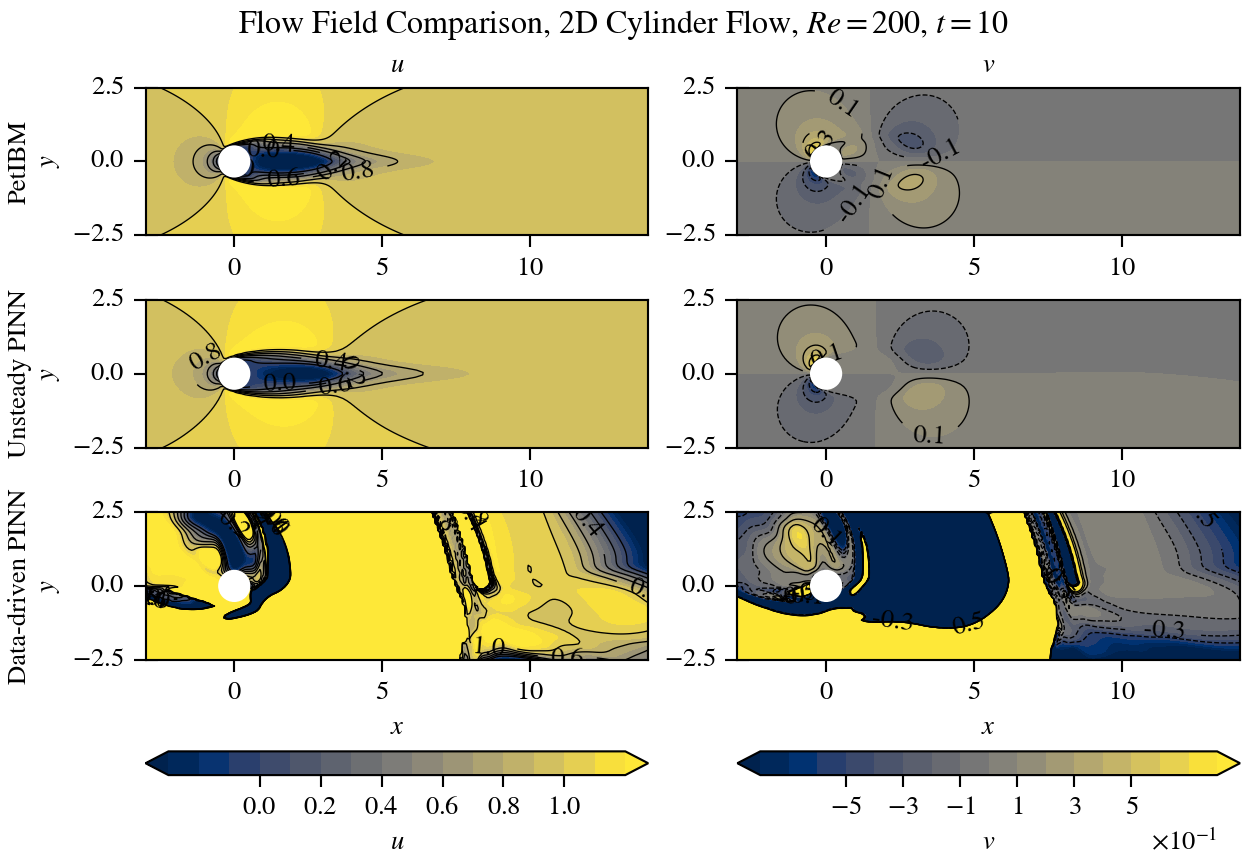
\includegraphics[width=0.9\linewidth]{cylinder-2d-re200/contour-comparison-uv-t10}
    \caption{PINNs, 2D Cylinder, $Re=200$: flow field comparisons for $u$ and $v$ at $t=10$}
    \label{fig:cylinder-re200-contour-uv-t10}
\end{figure}

\begin{figure}[hbt!]
    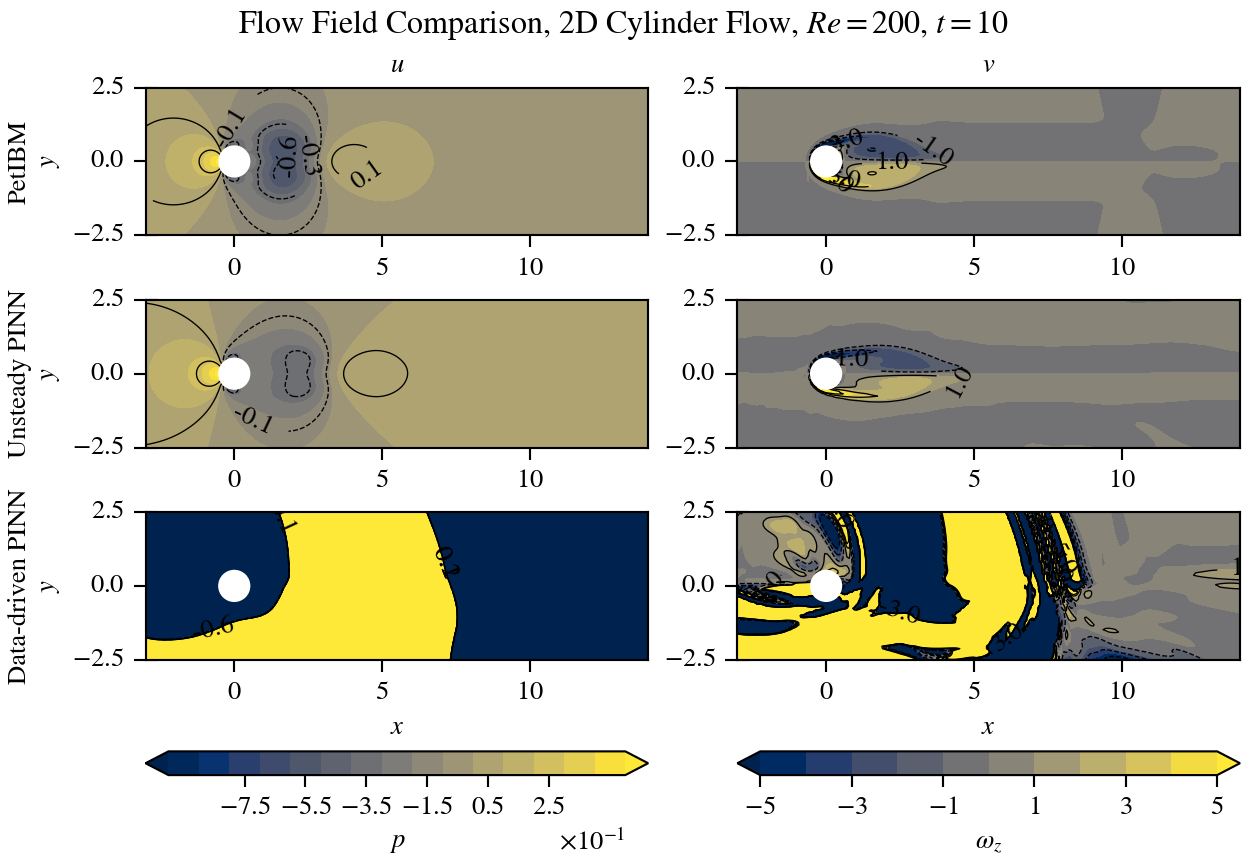
\includegraphics[width=0.9\linewidth]{cylinder-2d-re200/contour-comparison-pwz-t10}
    \caption{PINNs, 2D Cylinder, $Re=200$: flow field comparisons for $p$ and $\omega_z$ at $t=10$}
    \label{fig:cylinder-re200-contour-pwz-t10}
\end{figure}

\begin{figure}[hbt!]
    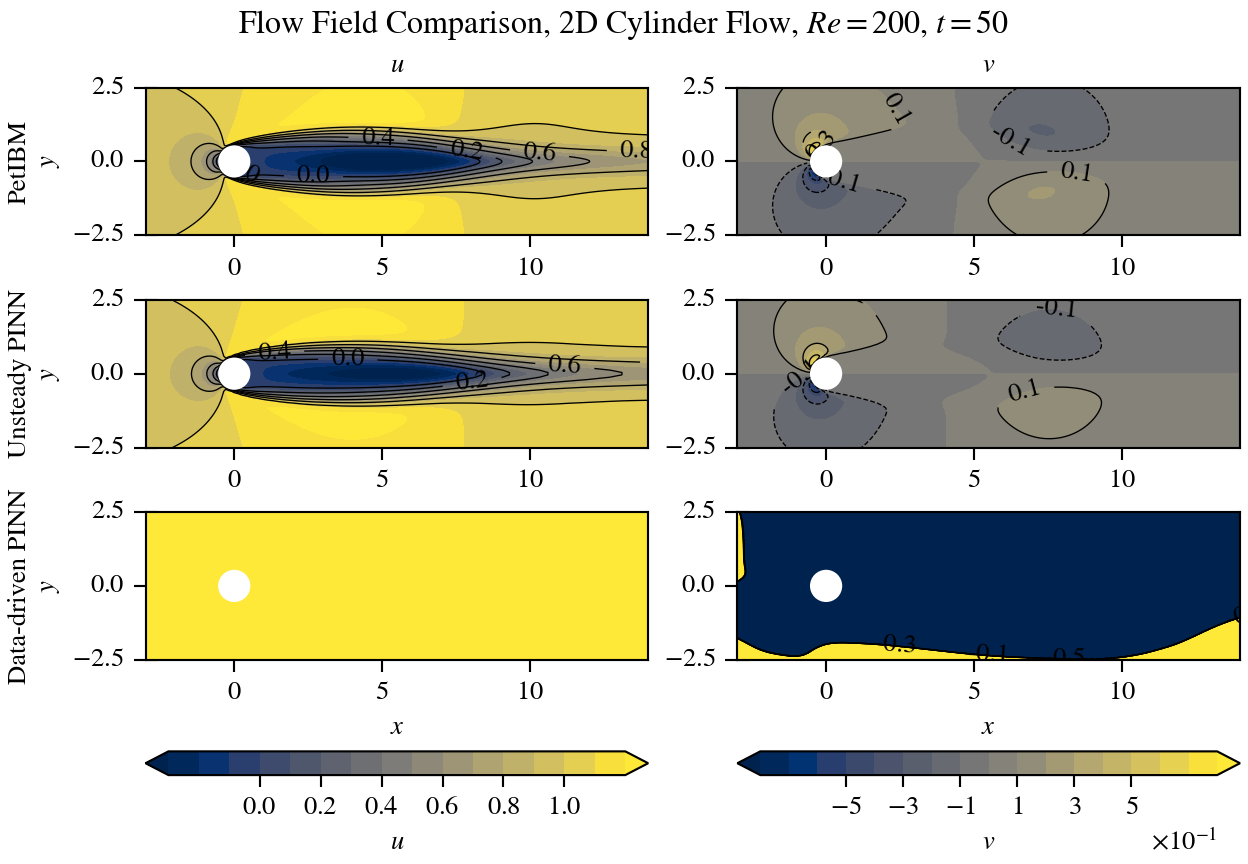
\includegraphics[width=0.9\linewidth]{cylinder-2d-re200/contour-comparison-uv-t50}
    \caption{PINNs, 2D Cylinder, $Re=200$: flow field comparisons for $u$ and $v$ at $t=50$}
    \label{fig:cylinder-re200-contour-uv-t50}
\end{figure}

\begin{figure}[hbt!]
    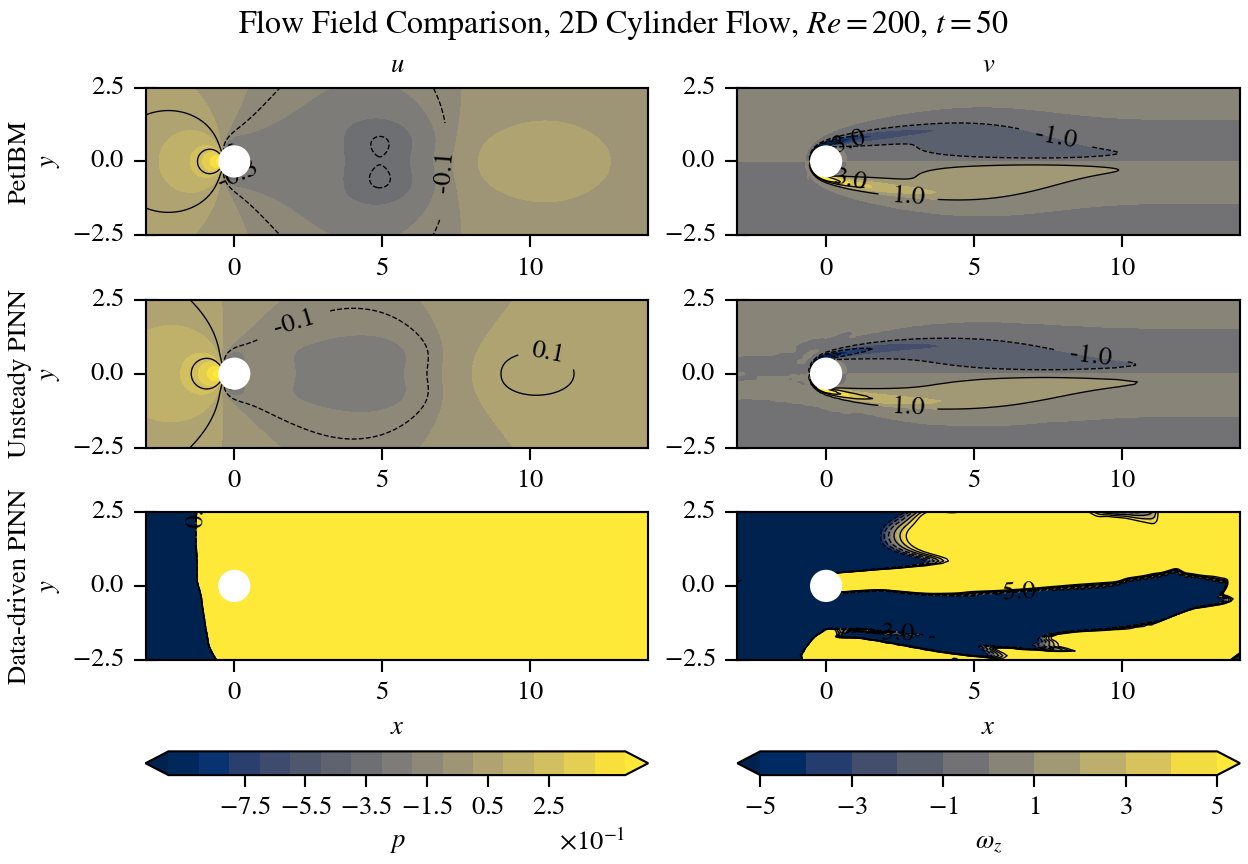
\includegraphics[width=0.9\linewidth]{cylinder-2d-re200/contour-comparison-pwz-t50}
    \caption{PINNs, 2D Cylinder, $Re=200$: flow field comparisons for $p$ and $\omega_z$ at $t=50$}
    \label{fig:cylinder-re200-contour-pwz-t50}
\end{figure}

\begin{figure}[hbt!]
    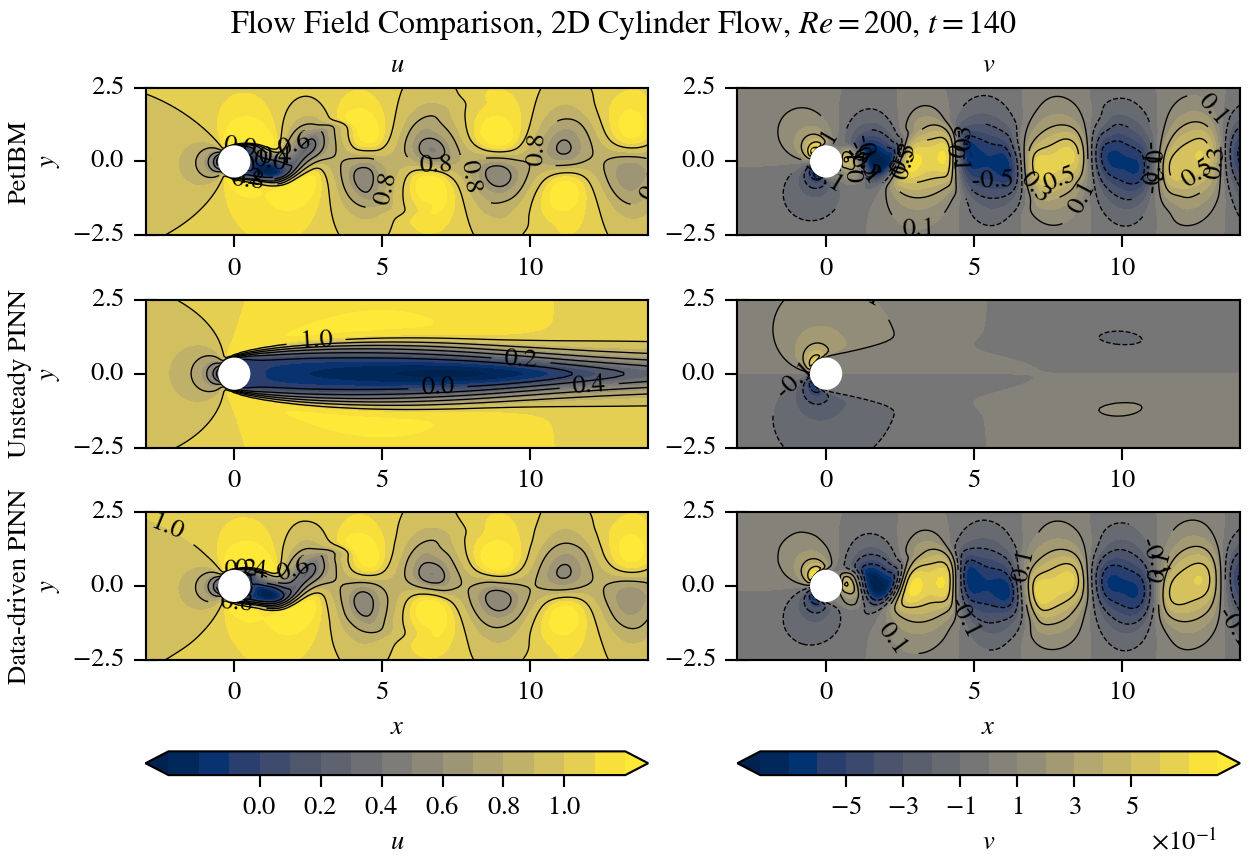
\includegraphics[width=0.9\linewidth]{cylinder-2d-re200/contour-comparison-uv-t140}
    \caption{PINNs, 2D Cylinder, $Re=200$: flow field comparisons for $u$ and $v$ at $t=140$}
    \label{fig:cylinder-re200-contour-uv-t140}
\end{figure}

\begin{figure}[hbt!]
    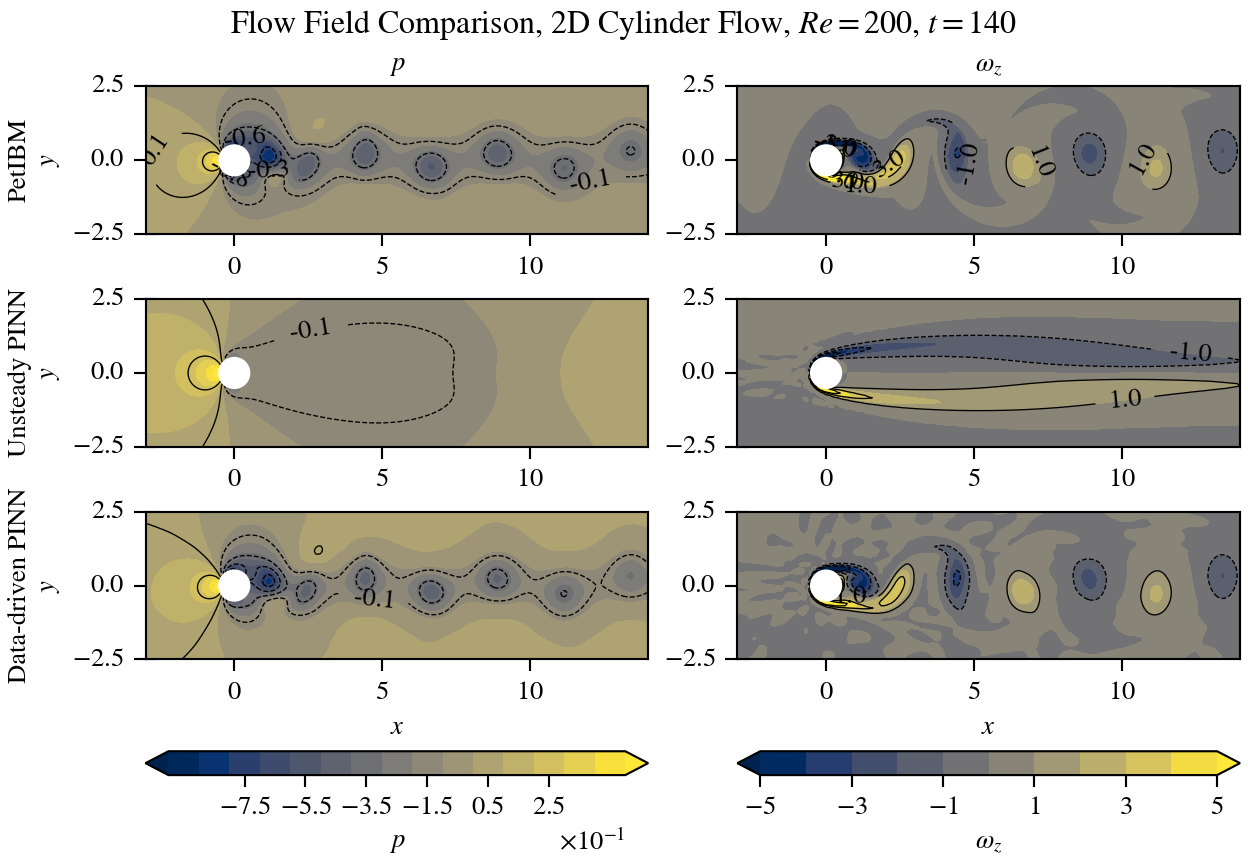
\includegraphics[width=0.9\linewidth]{cylinder-2d-re200/contour-comparison-pwz-t140}
    \caption{PINNs, 2D Cylinder, $Re=200$: flow field comparisons for $p$ and $\omega_z$ at $t=140$}
    \label{fig:cylinder-re200-contour-pwz-t140}
\end{figure}

\begin{figure}[hbt!]
    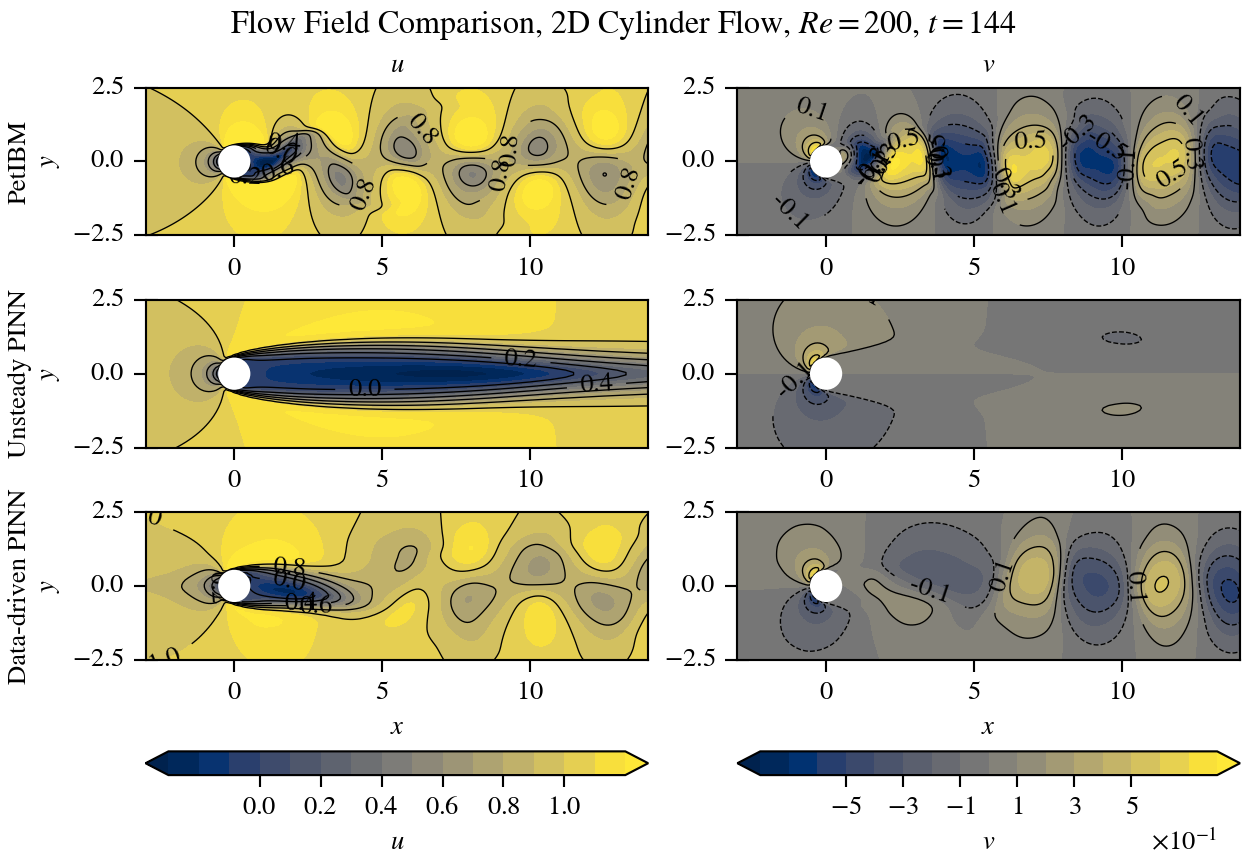
\includegraphics[width=0.9\linewidth]{cylinder-2d-re200/contour-comparison-uv-t144}
    \caption{PINNs, 2D Cylinder, $Re=200$: flow field comparisons for $u$ and $v$ at $t=144$}
    \label{fig:cylinder-re200-contour-uv-t144}
\end{figure}

\begin{figure}[hbt!]
    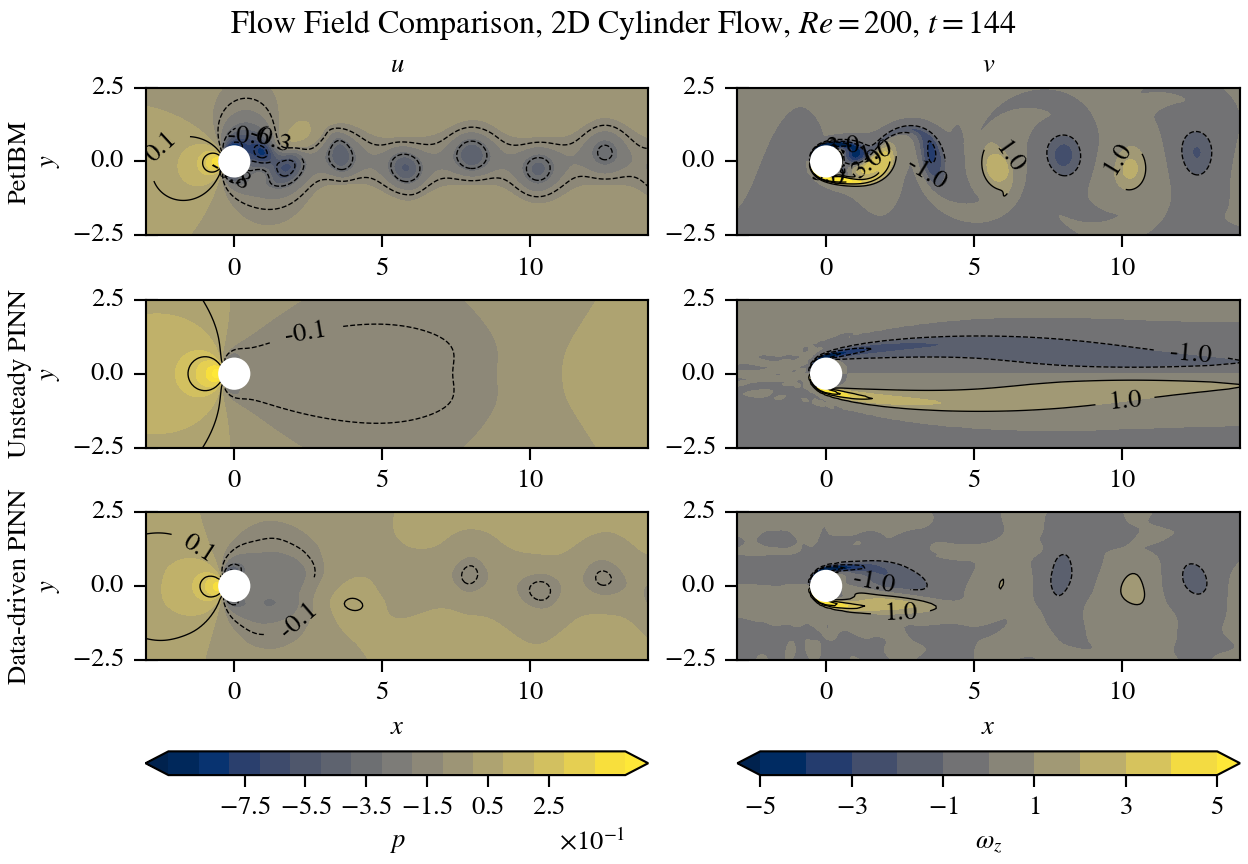
\includegraphics[width=0.9\linewidth]{cylinder-2d-re200/contour-comparison-pwz-t144}
    \caption{PINNs, 2D Cylinder, $Re=200$: flow field comparisons for $p$ and $\omega_z$ at $t=144$}
    \label{fig:cylinder-re200-contour-pwz-t144}
\end{figure}

\begin{figure}[hbt!]
    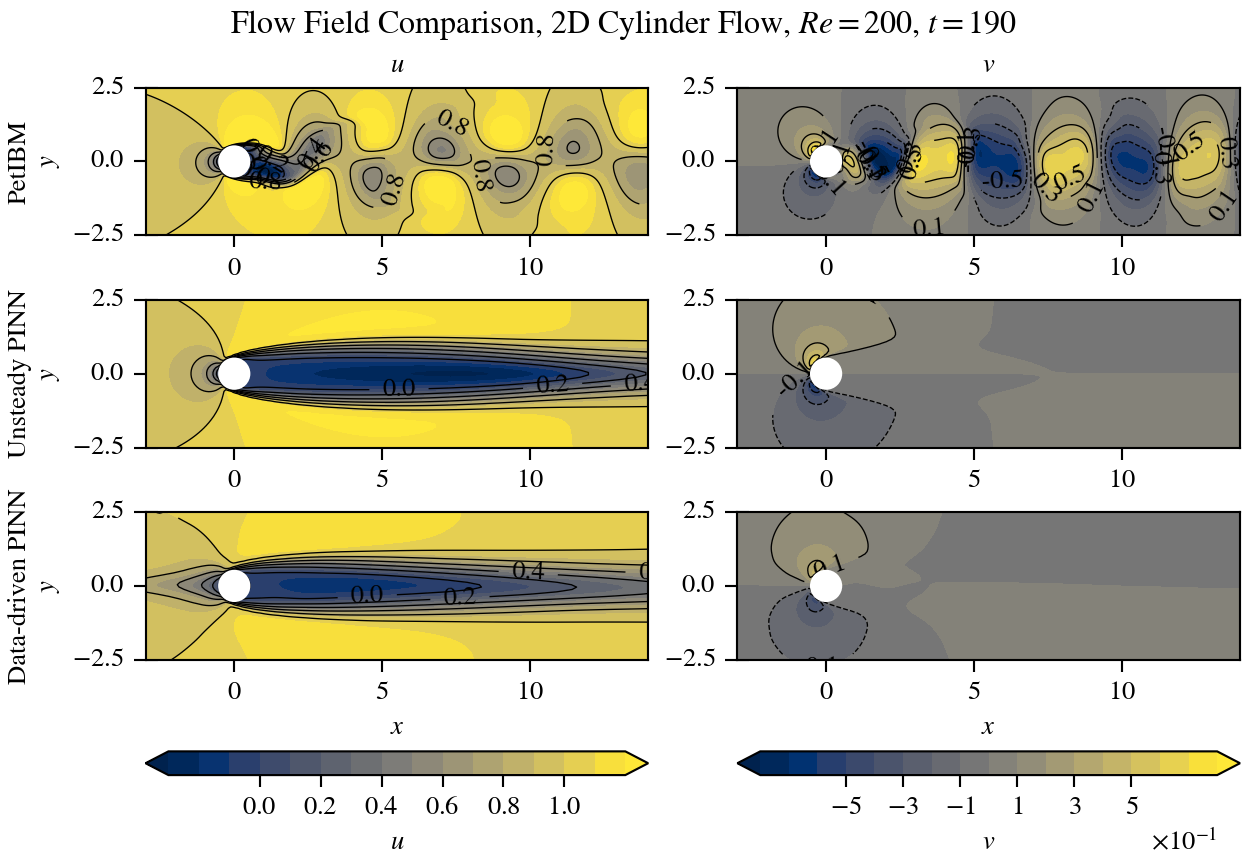
\includegraphics[width=0.9\linewidth]{cylinder-2d-re200/contour-comparison-uv-t190}
    \caption{PINNs, 2D Cylinder, $Re=200$: flow field comparisons for $u$ and $v$ at $t=190$}
    \label{fig:cylinder-re200-contour-uv-t190}
\end{figure}

\begin{figure}[hbt!]
    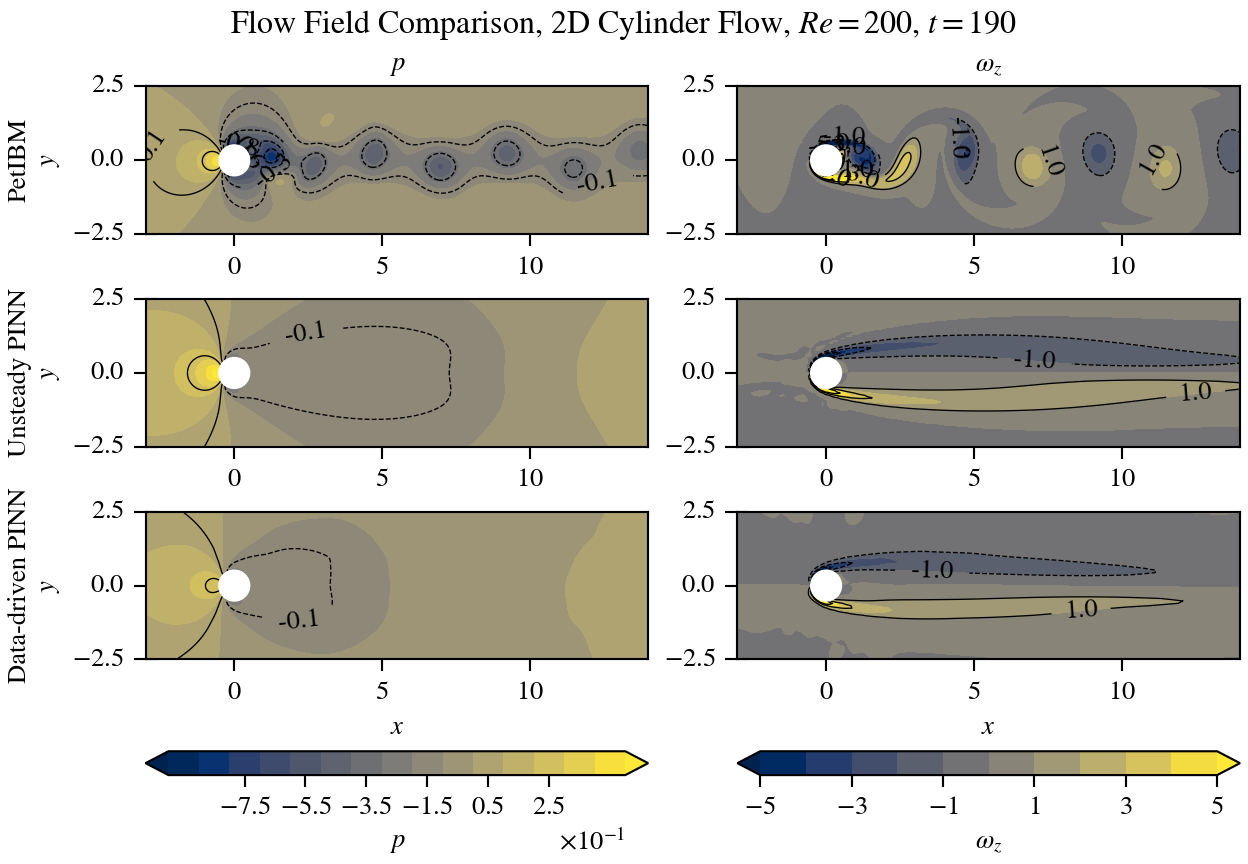
\includegraphics[width=0.9\linewidth]{cylinder-2d-re200/contour-comparison-pwz-t190}
    \caption{PINNs, 2D Cylinder, $Re=200$: flow field comparisons for $p$ and $\omega_z$ at $t=190$}
    \label{fig:cylinder-re200-contour-pwz-t190}
\end{figure}

The reason for the steady behavior of the unsteady PINN is unknown to us at this point.
A steady solution like we showed in these figures might still be physical in a perfect world when there is absolutely no perturbation and noise.
In the real world, the shedding is triggered by the natural perturbation.
In computer simulations, the shedding is triggered by all kinds of numerical errors, such as rounding errors and truncation errors.
These numerical errors mimic the natural perturbation.
As errors also exist in PINNs, PINNs are expected to develop vortex shedding.

In traditional numerical simulations, sometimes it is also difficult to develop vortex shedding especially if everything is symmetric.
However, we are still able to manually triggered shedding by using non-uniform ICs.
This did not happen to our benchmarks, either.
The data-driven PINN can be seen as a data-free PINN with non-uniform IC.
And given that this non-uniform IC already has shedding, the vortex shedding phenomenon is supposed to continue.
On the contrary, the data-driven PINN does not only stop generating new vortex but also falls back to the steady-state behavior.
At this point, we have not been able to determine the reason.

Aside from that the shedding does not continue after $t=140$ in the data-driven PINN, we are also not satisfied with its predictions before $t=125$.
Surely there were no training points before $t=125$ during the training.
However, one reason for using data-driven PINNs is to have a better prediction capability on new data that were not seen before.
In other words, we expected PINNs to have a satisfying extrapolation capability.
If data-driven PINNs do not perform well on extrapolation but can only handle interpolation problems, then its advantage over regular data-only machine learning may need more examination.

We must emphasize that while there are too many configurations and settings to try, our benchmark on data-driven PINNs may be very limited and naive.
Our focus in this work is still the data-free PINNs in solving PDEs.
% vim:ft=tex